\documentclass[10pt]{article}
\usepackage[margin=0.8in]{geometry}
\usepackage{amsmath,amssymb,booktabs,graphicx,adjustbox,float}
\usepackage[hidelinks]{hyperref}
\usepackage{caption,titlesec}
\captionsetup{font=small,labelfont=bf,skip=4pt}
\setlength{\intextsep}{8pt}
\titlespacing*{\section}{0pt}{1.4ex plus .2ex}{0.6ex}
\setlength{\parindent}{0pt}
\setlength{\parskip}{0.35em}
\setlength{\tabcolsep}{5pt}
\newcommand{\rt}[3]{\begin{table}[H]\centering\small\caption{#2}\label{#3}\begin{adjustbox}{max width=\linewidth}\input{results/brief_#1.tex}\end{adjustbox}\end{table}}
\title{Homework 1: Discrete State Dynamic Programming}
\author{Mishuk Roy}
\date{ECONS 509, Fall 2026}
\begin{document}
\begin{center}{\Large\bfseries Homework 1: Discrete State Dynamic Programming}\\[6pt]Mishuk Roy\\[3pt]ECONS 509, Fall 2026\end{center}
\section{Model and household solvers: part (a)}
I solve the household problem at fixed prices implied by $K^0=5$, with
$\beta=0.96$, $\sigma=1.5$, labor supply one, efficiency states $(0.8,1.2)$,
and $P_{ss'}=0.5$. With $(z,\alpha,\delta)=(1,0.36,0.1)$, the prices are
$w^0=1.1423762763$ and $r^0=0.0285173311$.
The Bellman and Euler derivations are in \texttt{manual/derivation.pdf}; numerical definitions follow \texttt{spec.md}.

The baseline uses $N=1000$ uniform points on $[0,20]$, zero initial values, and
\[
d(x)=\max_m\frac{|\mathcal T(x)_m-x_m|}{|x_m|+1}\leq10^{-8}.
\]
Counts include the stopping check; updates equal checks minus one.
\rt{solvers}{Baseline household solvers. Setup and solve times are separate.}{tab:solvers}
The contraction calculation $\log(10^{-8})/\log(0.96)=451.244$ predicts the scale
of an eight-order error reduction; VFI takes 379 checks. The difference reflects
the relative residual criterion, initial error, and realized contraction.
Howard evaluates each improved policy exactly and terminates after few policy
changes. Modified Howard uses $H=50$ inner evaluations per update, accelerating
convergence while avoiding a linear solve. Its 15 checks require 700 inner steps.
I select modified Howard, the fastest passing solver in these runs.

Fixed-step GD uses $\eta=5\times10^{-4}$, below the conservative local stability
limit $2/(1+\beta\sqrt{2000})^2\simeq0.00103623$; Adam uses learning rate $0.1$.
Both remain unconverged at 20,000 checks. For a fixed greedy policy, let
$J=I-\beta Q_G$. The assignment's lower-bound benchmark is
$\kappa(J^TJ)\geq(1-\beta)^{-2}=625$.
\rt{conditioning}{Local singular values and condition numbers, from \texttt{results/d\_theory.json}.}{tab:conditioning}
The severe conditioning at zero values is consistent with GD stalling. These
fixed-policy diagnostics do not guarantee global convergence. The Howard time
includes the first SciPy import, so timings describe the measured runs.

\section{Invariant distribution: parts (b)--(d)}
Using the same Howard policy, I solve $Q_G^T\pi=\pi$ with $\mathbf1^T\pi=1$
by power iteration, inverse iteration, and a normalized equation system.
\rt{distributions}{Dense and CSR distribution methods. Times exclude common matrix construction/conversion; residuals are $\|Q_G^T\pi-\pi\|_\infty$.}{tab:distributions}
The largest pairwise differences are $5.49004\times10^{-12}$ within dense,
$5.48995\times10^{-12}$ within CSR, and $5.49005\times10^{-12}$ across formats.
All pass the $10^{-8}$ agreement criterion and distribution checks. I select
CSR power iteration: it is the fastest passing option and uses 212 updates.
All subsequent experiments retain the chosen methods.

\section{Asset range and grid: parts (e)--(g)}
At $N=1000$, support means asset nodes with marginal probability above $10^{-12}$;
support share is their fraction of all nodes.
\rt{ranges}{Uniform-grid range trials. The accepted top-mass threshold is $10^{-12}$.}{tab:ranges}
I reject $k_{\max}=2$ and choose $k_{\max}=5$, the smallest tested range with
zero top mass and room above its support endpoint. Wider ranges reduce resolution
for a fixed number of nodes.

On $[0,5]$, I compare the uniform grid with the exp-log grid
\[
k_n=\exp\!\left[\frac{n-1}{N-1}\log(1+k_{\max})\right]-1,
\qquad n=1,\ldots,N.
\]
\rt{grids}{Grid comparison at $N=1000$; error statistics use positive-saving states.}{tab:grids}
I choose exp-log spacing for its lower mean and stationary-weighted errors,
accepting its higher overall maximum. Both grids have zero top mass.
\rt{nodes}{Exp-log refinement on $[0,5]$. Total numerical time excludes verification and plot export.}{tab:nodes}
I select $N=5000$: it has the lowest tested errors and an acceptable runtime of
4.36 seconds. Mean assets stabilize near 0.45. They need not equal $K^0$, because
prices are fixed. At $N=100$, one upper-bound choice is flagged, with top mass
$2.67276\times10^{-53}$; the finer grids have neither upper-bound choices nor top
mass. Figure~\ref{fig:grids} plots both shocks at every $N$; distribution curves
show joint masses, not densities. My dated October 1--2 choices are in \texttt{log.md}.

\clearpage
\section{Euler accuracy and tests: part (h)}
For positive savings, define
\[
c^{EE}_{n,s}=\left[\beta(1+r^0)\sum_{s'}P_{ss'}
(c^{next}_{n,s,s'})^{-\sigma}\right]^{-1/\sigma},
\qquad E_{n,s}=\left|1-\frac{c^{EE}_{n,s}}{c_{n,s}}\right|.
\]
The equality applies off the borrowing constraint and artificial upper bound;
discrete choices leave a residual. On $A=\{g_{n,s}>0\}$, normalize stationary
weights as $q_{n,s}=\pi_{n,s}/\sum_A\pi$. The weighted maximum is $\max_A(qE)$.
\rt{accuracy}{Selected $N=5000$ Euler errors. Support maximum restricts to positive-saving states with joint probability above $10^{-12}$.}{tab:accuracy}
Regressing log error on log maximum grid step gives slopes 1.01312 (mean) and
0.932503 (maximum). Figure~\ref{fig:accuracy} supports approximately first-order
scaling over these grids; it does not establish an asymptotic theorem.
\rt{checks}{Final-grid numerical checks. All meet their registered criteria.}{tab:checks}
The selected household solve uses 14 checks, 13 updates, and 650 inner steps,
with $d(x)=6.31419\times10^{-9}$; power iteration uses 168 updates.
The agent's final audit records 484 passes, zero failures, and zero pending checks.
Its clean-copy reproduction matches the saved numerical outputs exactly.

\section{Independent verification and AI use}
The \textbf{2026-10-02 --- Mishuk verification results} entry in \texttt{log.md}
records two personal checks: the $N=100$ manual-kernel comparison gives 492 checks
in both implementations, maximum value difference $1.42\times10^{-14}$, and zero
policy mismatches; the saved-output calculations give zero budget discrepancy,
distribution sum 1.0, and Euler-error agreement within $2.22\times10^{-16}$.
The October 1--2 Codex entries document its automated tests, experiments, and
reproduction. Those agent measurements are distinct from my dated personal checks.

Codex (GPT-6; exact build unavailable) worked with Full Access to the repository,
implementing solvers and tests, running experiments, and producing outputs.
I supplied the inputs and manual reference, selected methods and grids, and recorded
personal verification. ChatGPT assisted with the report-check prompt, drafted and
shortened this report, checked saved numbers, and prepared tables, plots, and the
PDF. This report is AI-assisted and remains subject to my final review.

\clearpage
\appendix
\section{Required numerical figures}
\begin{figure}[H]\centering
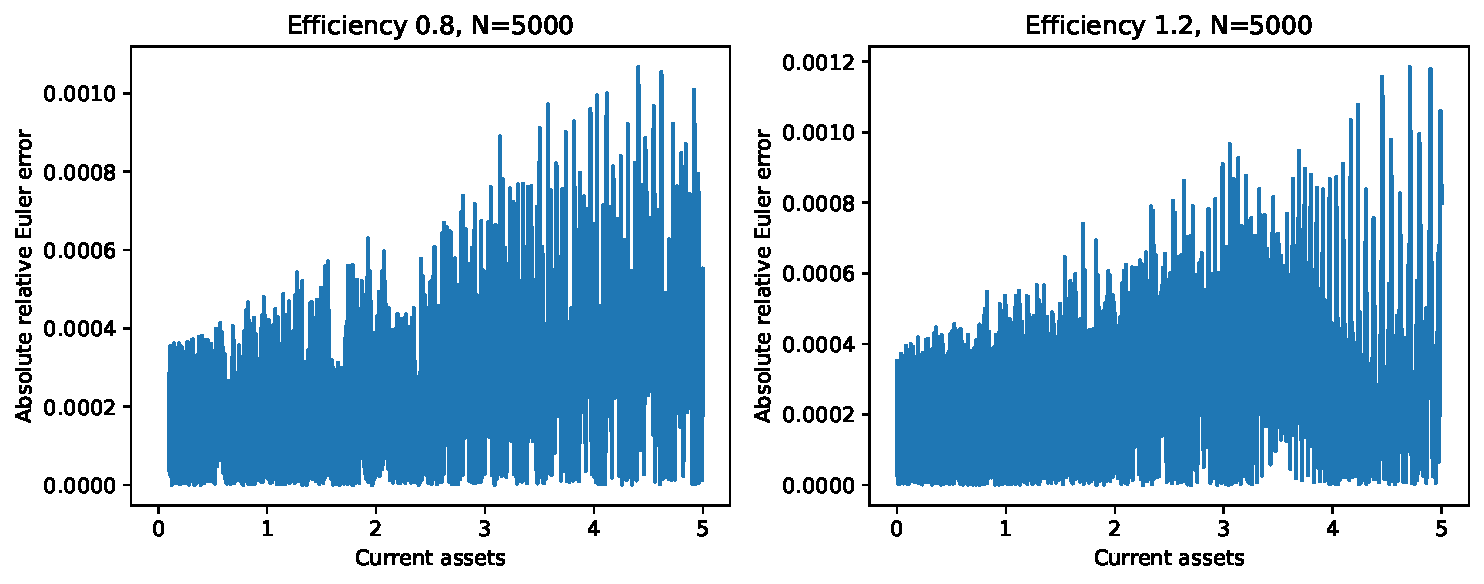
\includegraphics[width=0.93\linewidth]{results/h_euler.pdf}\par\medskip
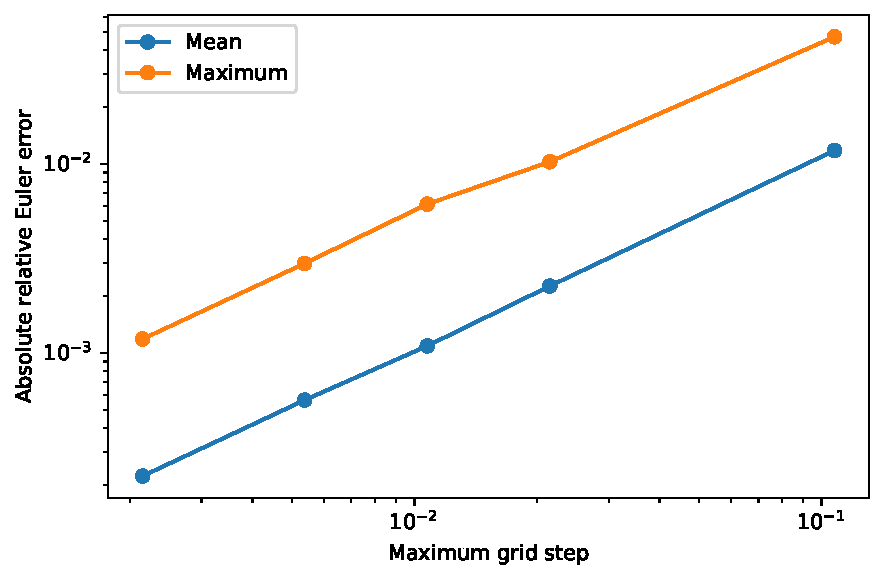
\includegraphics[width=0.88\linewidth]{results/h_scaling.pdf}
\caption{Selected-grid Euler residuals (top) and their scaling across all five grids (bottom).}
\label{fig:accuracy}
\end{figure}
\clearpage
\begin{figure}[H]\centering
\includegraphics[width=\linewidth]{results/brief_V.pdf}\par\medskip
\includegraphics[width=\linewidth]{results/brief_g.pdf}\par\medskip
\includegraphics[width=\linewidth]{results/brief_pi.pdf}
\caption{Values, savings policies, and joint invariant masses for both shocks, using every saved node at $N=100,500,1000,2000,5000$. Overlapping curves reflect close solutions.}
\label{fig:grids}
\end{figure}
\end{document}
